
\chapter{Machine learning e reti neurali}

% Possibile introduzione al machine learning generico

All'interno del complesso insieme di algoritmi ascrivibili all'ambito del Machine Learning, una delle classi più promettenti al fine di effettuare operazioni di regressione si rivela essere quella delle \emph{reti neurali}. Questi modelli, infatti, data la loro struttura, sono in grado di analizzare enormi quantità di dati non elaborati, identificando autonomamente pattern complessi, spesso fortemente non lineari, ed appredendo da essi. 

L'ispirazione alla base di tali algoritmi proviene dal funzionamento del cervello umano, in grado di analizzare in pochi millisecondi problemi complessi e, sfruttando anche informazioni passate immagazzinate all'interno delle singole sinapsi, generare una risposta ottimale. Naturalmente, replicarne la capacità di ricordare nel tempo grandi quantità di dati e l'elevato numero di interconnessioni, che definiscono con che livello di sofisticatezza si svolgono le operazioni necessarie, è quasi impossibile, data l'enorme potenza di calcolo che sarebbe necessaria. Tuttavia, le reti neurali sono in grado di migliorare con l'esperienza, analogamente al cervello, in una fase definita training e risultano persino più rapide nel processare le informazioni. 

A livello strutturale, quindi, l'elemento elementare risulta essere il \emph{neurone}, in grado di ricevere in input molteplici dati, elaborarli internamente tramite l'utilizzo di una funzione lineare, caratterizzata da specifici pesi e bias, e, in base alla funzione di attivazione prescelta, produrre un output. Solitamente si generano dei cosiddetti \emph{layer di neuroni}, che si interfacciano vicendevolmente. Una rete neurale, per essere definita tale, deve avere almeno due layer fondamentali: l'\emph{input layer}, che riceve direttamente i dati grezzi forniti all'algoritmo, e l'\emph{output layer}, che produce il risultato ricercato. Normalmente, tuttavia, a questi si aggiungono uno o più layer intermedi, definiti \emph{hidden layers}. Essi, infatti, sono necessari per aumentare  la capacità della rete di estrarre relazioni non lineari dai dati, pur aumentando la complessità e la potenza di calcolo associati al modello. Inoltre, in caso siano presenti almeno 3 layer complessivi, non ci si riferisce più all'ambito del semplice machine learning, bensì si entra in quello che viene definito \textbf{deep learning}.   

\begin{figure}[h!]
    \centering
    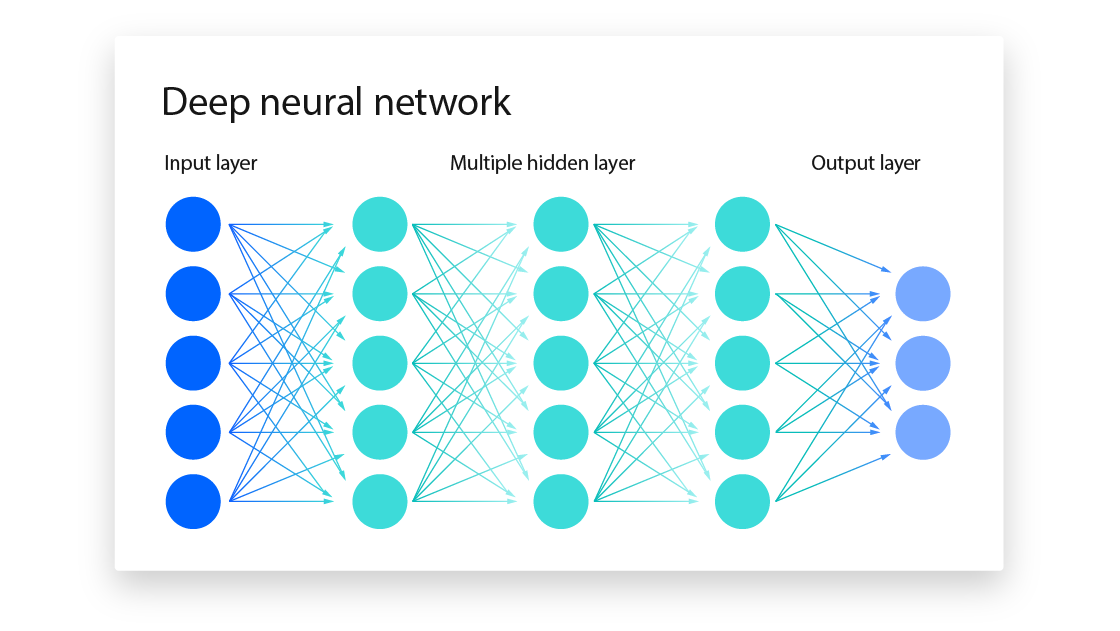
\includegraphics[width=0.8\linewidth]{images/NN/Struttura_base_DL.png}
    \caption{Struttura tipica di un algoritmo di Deep Learning\cite{IBM_NN}}
    \label{fig:DL_struct}
\end{figure}

% Qui si potrebbe aggiungere anche uno schema di funzionamento e spiegazione di forward e back propagation

\section{Elementi rete neurale}

Conclusa questa prima introduzione alle reti neurali, presentata schematicamente in \emph{Figura} \ref{fig:DL_struct}, è necessario analizzarne il funzionamento più nel dettaglio, in modo tale da comprendere, anche a livello matematico, come si arriva all'output desiderato. Nelle sezioni che seguiranno, pertanto, verranno descritti e valutati individualmente tutti gli elementi che compongono una rete neurale. 

\subsection{Neuroni}

Come anticipato, l'entità fondamentale di una rete neurale è il neurone, che risulta estremamente simile a livello concettuale rispetto alla controparte biologica, come si può notare dal confronto mostrato in \emph{Figura} \ref{fig:confronto_neuroni}. Più dettagliatamente, un neurone tradizionale riceve informazioni da altri neuroni tramite i dendriti, le elabora internamente e produce un output sotto forma di impulsi eletttrici, trasmessi ad altri elettroni attraverso le sinapsi poste alla fine della coda. Particolare attenzione va riservata al meccanismo di trasmissione delle informazioni, che avviene grazie a dei messaggeri chimici, chiamati \textit{neurotrasmettitori}, generati a partire dal segnale elettrico prima di giungere alle sinapsi. 

Un neurone artificiale, pur non necessitando della presenza di tutti questi elementi complessi, è in grado di replicare fedelmente il comportamento appena descritto. Ogni neurone, infatti, riceve informazioni da tutti i neuroni del layer che lo precede, le elabora tramite l'utilizzo di una funzione lineare e di una funzione di attivazione e produce un singolo output, trasmesso al layer successivo. Naturalmente, analogamente a ciò che avviene nel cervello umano, non tutti i percorsi tra neuroni impattano allo stesso modo per giungere al miglior output possibile. Ogni connessione, pertanto, presenta uno specifico peso $w_{i}$, determinato durante la fase di apprendimento della rete. 

Un neurone, pertanto, produce un primo output $z$ effettuando una somma pesata degli $n$ valori ricevuti in input:

    \begin{center}
        $z = \sum_{i=1}^{n} w_{i}*x_{i} + b$ \ \ \ $(2.1)$
    \end{center}

All'interno di questa relazione, sviluppata da Rosenblatt per il Perceptron, una delle prime reti neurali, compare un termine aggiuntivo oltre ai pesi, noto come \textit{bias}. Anch'esso viene modificato durante la fase di addestramento della rete al fine di ottimizzare il risultato del modello. 

\begin{figure}[h!]
    \centering
    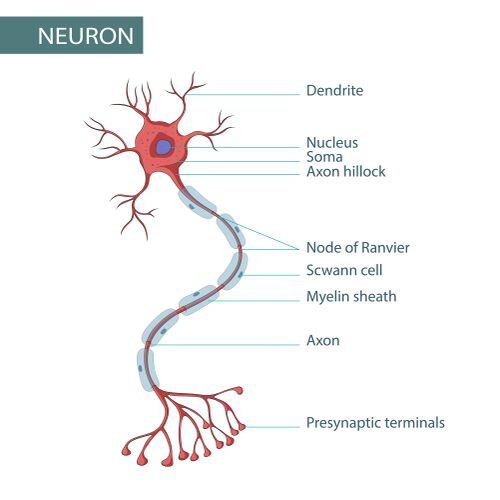
\includegraphics[width=0.5\linewidth]{images/NN/Neurone_bio_2.png}
    \caption{Confronto tra neurone biologico\cite{jpg_neurone_bio} e artificiale}
    \label{fig:confronto_neuroni}
\end{figure}


\subsection{Funzione di attivazione}

L'output prodotto nella prima fase di analisi da parte del neurone, necessita di un ulteriore passaggio prima di essere trasmesso ai layer successivi. Occorre, infatti, normalizzare il valore ottenuto e aggiungere non linearità al modello, potendo così approssimare pattern più complessi.

% Classificazione attivazione

\subsection{Learning Rule}



\section{Algoritmi tipici}